\section{Results}


\subsection{Optic Microscopy}

\begin{figure}[h!]
	\begin{center}
		\begin{tabular}{cc}
			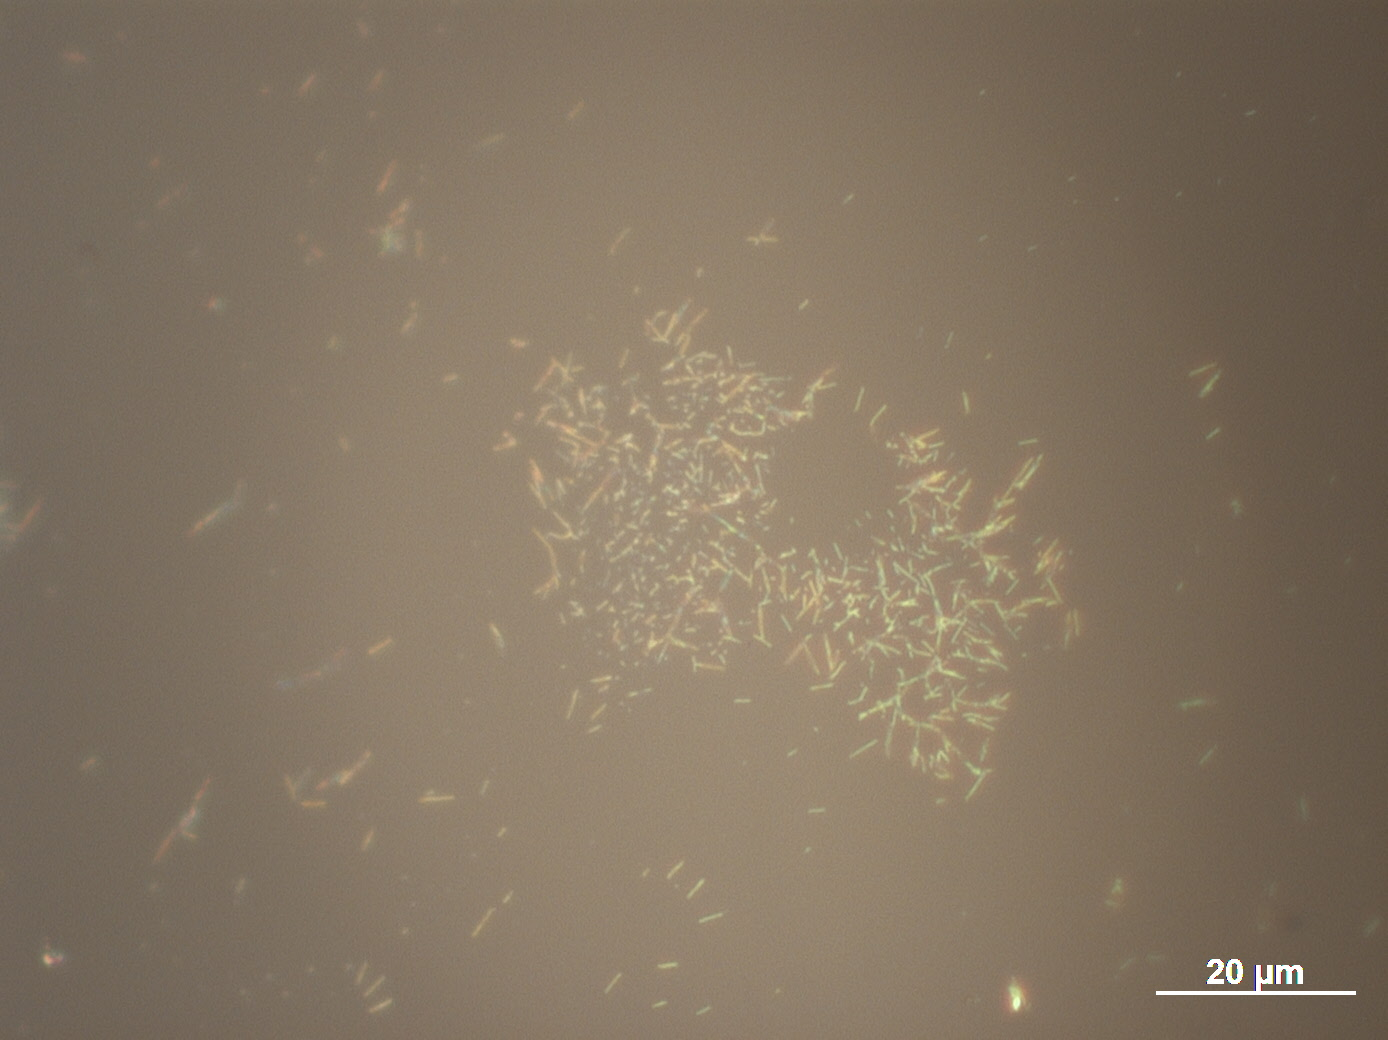
\includegraphics[width=7cm]{optic} &   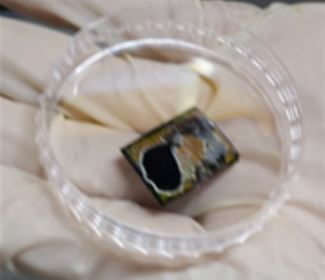
\includegraphics[width=7cm]{crystal}
		\end{tabular}
		\caption{The $^{12}$CO J = 2 - 1 intensity contour map (left) and the line profile (right) of FIR2.}	
		\label{fig:FIR221}
	\end{center}
\end{figure}


\newpage
\subsubsection{X-Ray Diffraction}

\clearpage
\newpage
\subsection{TRPL spectroscopy}

TRPL 그래프는 위의 그림과 같이 파란색의 그래프이다. t=28ns부근에서 최댓값을 확인 할 수 있었고, 그 시간 이후의 데이터를 시간에 따른 지수 함수(exponential function)들의 합으로 fitting 할 수 있는데, 그 식은 $\sum_{i}^{} {e}^{-t/{\tau}_{i}}$ 로 표현된다. CsPbBr3는 exciton과 biexciton의 recombination으로 나뉘기 때문에 두 개의 exponential function의 합으로 표현하였다. 

그래프의 피팅을 위해 파이썬을 활용하였다. TRPL 데이터를 순서쌍으로 바꿔서 그래프를 그린 후, 파이썬에 내재된 함수인 curve fit을 이용하여 최소제곱법으로 가장 비슷한 함수를 찾아낸다. 

만들어진 결정이 CsPbBr3 임을 확인하기 위해서 exciton과 biexciton의 recombination rate에 대한 비율을 계산하였다. 
ND0 필터를 사용했을 때 두 recombination rate 사이의 비율에 대한 평균값은 3.43 이었고 ND1필터를 사용 했을 때는 3.30이었다.